\documentclass[a4paper,14pt]{extarticle}

\usepackage[left=30mm, right=10mm, top=20mm, bottom=20mm]{geometry}

\usepackage{amssymb}
\usepackage{amsmath}
\usepackage{tikz}
\usepackage{pgfplots}

\usepackage{graphicx}
\usepackage{setspace}

\usepackage{minted}
\usepackage{xcolor}

\usepackage{siunitx}
\usepackage{booktabs}

\usepackage[T2A]{fontenc}
\usepackage[utf8]{inputenc}
\usepackage[russian]{babel}
\usepackage{tempora}
\usepackage{type1cm}
\usepackage{indentfirst}

\usepackage{amssymb}
\usepackage{amsmath}
\usepackage{tikz}
\usepackage{pgfplots}
\usepackage{graphicx}
\usepackage{caption}
\usepackage{subcaption}
\usepackage[hidelinks]{hyperref}
\usepackage[russian]{cleveref}
\usepackage{bookmark}

\renewcommand{\theFancyVerbLine}{%
	\sffamily\small\color{black}\arabic{FancyVerbLine}%
}

\definecolor{codebg}{rgb}{0.12,0.12,0.14}
\definecolor{codeframe}{rgb}{0.40,0.40,0.45}
\definecolor{keywordcolor}{rgb}{0.45,0.65,1.0}
\definecolor{stringcolor}{rgb}{1.0,0.55,0.45}
\definecolor{commentcolor}{rgb}{0.55,0.75,0.60}
\definecolor{textcolor}{rgb}{0.90,0.90,0.90}

\setminted{
    bgcolor=codebg,
	fillcolor=codebg,
	framesep=1em,
	frame=single,
    rulecolor=\color{codeframe},
    fontsize=\normalsize,
    baselinestretch=1.1,
    linenos,
    numbersep=6pt,
    tabsize=4,
    breaklines,
    breakbytoken,
	breaksymbolleft={},
    autogobble,
    showspaces=false,
    showtabs=false,
}

\usemintedstyle{lightbulb}
\setmintedinline{
    bgcolor=codebg
}

\makeatletter
\setlength{\@fptop}{0pt}
\setlength{\@fpsep}{8pt}
\setlength{\@fpbot}{0pt plus 1fil}
\makeatother

\DeclareMathOperator{\Uniform}{U}
\DeclareMathOperator{\Bernoulli}{Bernoulli}
\DeclareMathOperator{\Bin}{Bin}
\DeclareMathOperator{\N}{N}


\begin{document}
    \begin{titlepage}
		\centering
		
		
\includegraphics{images/FEFU-logo.jpg}\\
		МИНИСТЕРСТВО ОБРАЗОВАНИЯ И НАУКИ РОССИЙСКОЙ ФЕДЕРАЦИИ\\
		Федеральное государственное автономное образовательное учреждение высшего образования\\
		\textbf{«Дальневосточный федеральный университет»}

		\rule{\linewidth}{0.8mm}\\[0.3cm]
		
		\textbf{ИНСТИТУТ МАТЕМАТИКИ И КОМПЬЮТЕРНЫХ ТЕХНОЛОГИЙ}\\
		\textbf{Кафедра математического и компьютерного моделирования}\\
		\vspace*{0.9cm}
		
		Кулахсзян Сергей Грайрович\\
        \vspace*{0.3cm}

		ВЫБОРКА \\
		\vspace*{0.3cm}

		\textbf{ЛАБОРАТОРНАЯ РАБОТА № 1}\\
		\vspace*{0.3cm}
		
		Направление подготовки 02.03.01сцт Сквозные цифровые технологии,\\ 
        бакалавриатская программа «Математика и компьютерные науки»\\ 
        Очной формы обучения\\
		\vspace{1.5cm}

		
		\vfill
		\centering
		г. Владивосток\\
		2026
	\end{titlepage}

    \tableofcontents
	\newpage

    \section{Генерация выборок}

    Равномерное распределение $X \sim \Uniform(a = -1, b = 4)$:

    \begin{minted}{python}
        data["uniform"][100]["X"] = stats.uniform.rvs(loc=-1, scale=5, size=100, random_state=random_state)
        data["uniform"][1000]["X"] = stats.uniform.rvs(loc=-1, scale=5, size=1000, random_state=random_state)
    \end{minted}

    Распределение Бернулли $X \sim \Bernoulli(p = 0.25)$:
    \begin{minted}{python}
        data["bernoulli"][100]["X"] = stats.bernoulli.rvs(p=0.25, size=100, random_state=random_state)
        data["bernoulli"][1000]["X"] = stats.bernoulli.rvs(p=0.25, size=1000, random_state=random_state)
    \end{minted}

    Биномиальное распределение $X \sim \Bin(n = 17, p = 0.25)$:
    \begin{minted}{python}
        data["binom"][100]["X"] = stats.binom.rvs(p=0.25, n=17, size=100, random_state=random_state)
        data["binom"][1000]["X"] = stats.binom.rvs(p=0.25, n=17, size=1000, random_state=random_state)
    \end{minted}

    Нормальное распределение $X \sim \N(M = 15, \sigma = 5)$:
    \begin{minted}{python}
        data["norm"][100]["X"] = stats.norm.rvs(loc=15, scale=5, size=100, random_state=random_state)
        data["norm"][1000]["X"] = stats.norm.rvs(loc=15, scale=5, size=1000, random_state=random_state)
    \end{minted}

    \section{Реализация выборочных характеристик}

    Выборочное среднее:\\
    $\displaystyle \overline{x}_B = \sum_{i = 1}^{n} \frac{x_i}{n}$

    \begin{minted}{python}
        def mean(x: list[float]) -> float:
            return sum(x) / len(x)
    \end{minted}

    Выборочная дисперсия:\\
    $\displaystyle D_B = \sum_{i = 1}^{n} \frac{(x_i - \overline{x}_B)^2}{n}$

    \begin{minted}{python}
        def dispersion(x: list[float]) -> float:
            x_mean = mean(x)
            return sum((x_i - x_mean) ** 2 for x_i in x) / len(x)
    \end{minted}

    Выборочное стандартное отклонение:\\
    $\displaystyle \sigma_B = \sqrt{D_B}$

    \begin{minted}{python}
        def standard_deviation(x: list[float]) -> float:
            return dispersion(x) ** 0.5
    \end{minted}

    \section{Сравнение расчетных характеристик}

    \begin{table}[h!]
        \centering
        \label{tab:results_lines}
        \small
        % Символ | между буквами l и c создает вертикальную линию
        \begin{tabular}{|l|c|c|c|c|c|c|}
            \hline
            \textbf{№ выборки} & \multicolumn{2}{c|}{\textbf{Среднее}} & \multicolumn{2}{c|}{\textbf{Дисперсия}} & \multicolumn{2}{c|}{\textbf{Ст. отклонение}} \\
            \cline{2-7} % Линия для колонок со 2 по 7
            (распределение-размер) & моё & numpy & моя & numpy & моё & numpy \\
            \hline
            № 1 (равномерное-100)  & 1.4937 & 1.4937 & 2.1570 & 2.1570 & 1.4687 & 1.4687 \\ \hline
            № 2 (равномерное-1000) & 1.4820 & 1.4820 & 2.0780 & 2.0780 & 1.4415 & 1.4415 \\ \hline
            № 3 (Бернулли-100)     & 0.2700 & 0.2700 & 0.1971 & 0.1971 & 0.4440 & 0.4440 \\ \hline
            № 4 (Бернулли-1000)    & 0.2440 & 0.2440 & 0.1845 & 0.1845 & 0.4295 & 0.4295 \\ \hline
            № 5 (биномиальное-100) & 4.2600 & 4.2600 & 3.6124 & 3.6124 & 1.9006 & 1.9006 \\ \hline
            № 6 (биномиальное-1000)& 4.2290 & 4.2290 & 3.2526 & 3.2526 & 1.8035 & 1.8035 \\ \hline
            № 7 (нормальное-100)   & 15.9197 & 15.9197 & 30.4590 & 30.4590 & 5.5190 & 5.5190 \\ \hline
            № 8 (нормальное-1000)  & 14.9599 & 14.9599 & 26.9451 & 26.9451 & 5.1909 & 5.1909 \\ \hline
        \end{tabular}
    \end{table}

    \section{Построение графиков}

    Для начало определяется длина частотного интервала:\\
    $\displaystyle
    h = \frac{R}{k} \\
    R = X_{\max} - X_{\min} \\
    k = 1 + 3.322 \lg n \\
    $
    Тут $R$ -- размах, $k$ -- число частотных интервалов, $h$ -- длина частотного интервала

    Для каждого частотного интервала $[X_{\min} + ih; X_{\min} + (i + 1)h], i = \overline{0, k}$ определяется значение относительной частоты: \\
    $\displaystyle w_i = \frac{m_i}{n}$,\\
    где $m_i$ -- частота вхождений элементов выборки в частотный интервал $[X_{\min} + ih; X_{\min} + (i + 1)h]$, $n$ -- объём выборки.

    Плотность относительной частоты тогда будет равна:\\
    $\displaystyle h_i = \frac{w_i}{h}$

    Таким образом в гистограмме для каждого частотного интервала будет определён $h_i$

    \subsection{Равномерное распределение}

    Плотность распределений для равномерного распределения имеет вид:\\
    $\displaystyle f_X(x) = \frac{1}{b - a}$

    Код построения графиков будет иметь вид:
    \begin{minted}{python}
        def f_x(x: float) -> float:
            return 1 / (4 + 1)

        fig, axes = plt.subplots(1, 2)

        for col, size in enumerate([100, 1000]):
            ax = axes[col]
            sample = data["uniform"][size]["X"]

            k = int(1 + 3.322 * np.log10(len(sample)))
            h = (max(sample) - min(sample)) / k

            endpoints = np.linspace(min(sample), max(sample), k + 1)
            heights = []
            for i in range(k):
                left = endpoints[i]
                right = endpoints[i+1]
                count = ((sample >= left) & (sample < right)).sum()
                
                density_height = count / (size * h)
                heights.append(density_height)

            bin_centers = endpoints[:-1] + h / 2
            ax.bar(bin_centers, heights, width=h, alpha=0.5, edgecolor='black')

            k = np.linspace(-1, 4, 100)
            ax.plot(k, [f_x(i) for i in k], 'r-', lw=2.5, label='Плотность вероятностей')

            ax.set_title(f"Равномерное-{size}")
            ax.set_ylabel("Плотность")
            ax.legend(fontsize='small')
            ax.grid(axis='y', alpha=0.3)
    \end{minted}

    Сами графики получились такими:
    \begin{figure}[ht!]
        \centering
        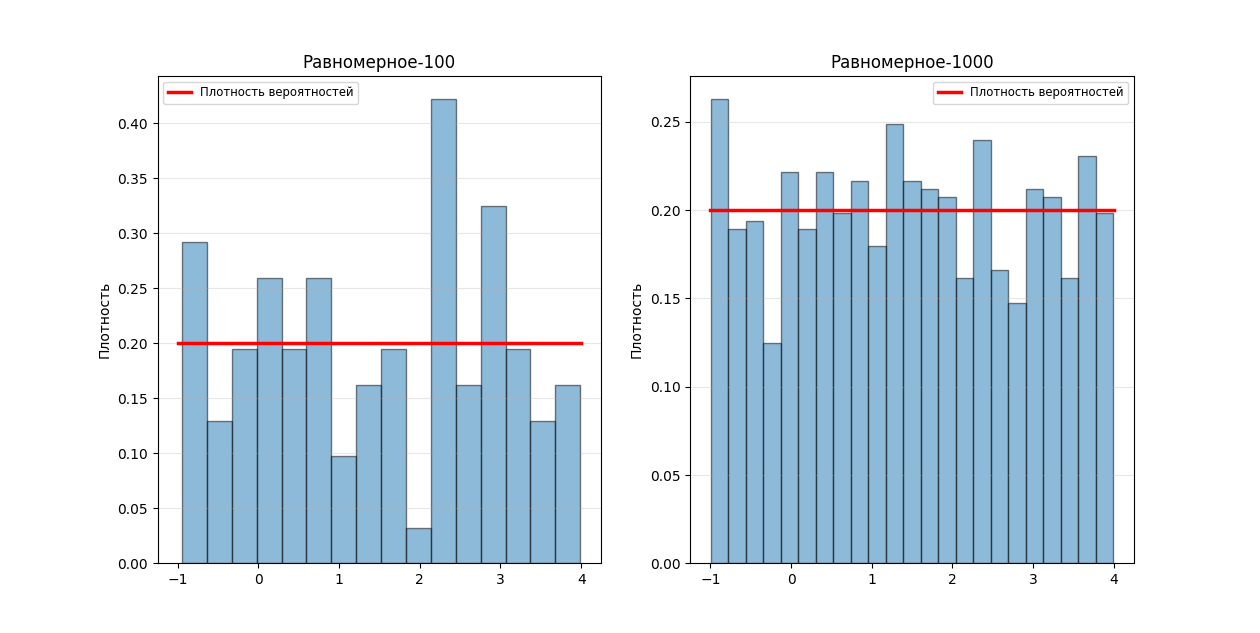
\includegraphics[width=\textwidth]{images/uniform.png}
        \label{fig:uniform_100}
    \end{figure}

    \subsection{Распределение Бернулли}

    В случае распределения Бернулли случайная величина может принимать только 2 значения: 0 и 1.
    В связи с этим $k = 2$, то бишь будет частотный интервал для 0 и 1.

    Функция вероятности распределения Бернулли имеет вид: \\
    $\displaystyle 
    f_X(x) = \begin{cases}
        p, & \text{если } x = 1 \\
        1 - p, & \text{если } x = 0 \\
        0, & \text{иначе}
    \end{cases}$

    Таким образом код выглядит так:
    \begin{minted}{python}
        fig, axes = plt.subplots(1, 2)

        for col, size in enumerate([100, 1000]):
            ax = axes[col]
            sample = data["bernoulli"][size]["X"]

            m_1 = sum(sample)
            m_0 = size - m_1
            
            w_0 = m_0 / size
            w_1 = m_1 / size

            heights = [w_0, w_1]

            ax.bar([0, 1], heights, width=1, alpha=0.5, edgecolor='black')

            ax.scatter([0, 1], heights, s=100, zorder=5, label='Функция вероятности', color="red")
            ax.plot([0, 1], heights, color="red")

            ax.set_title(f"Бернулли-{size}")
            ax.set_ylabel("Плотность")
            ax.legend(fontsize='small')
            ax.grid(axis='y', alpha=0.3)
    \end{minted}

    График будет выглядеть так:
    \begin{figure}[ht!]
        \centering
        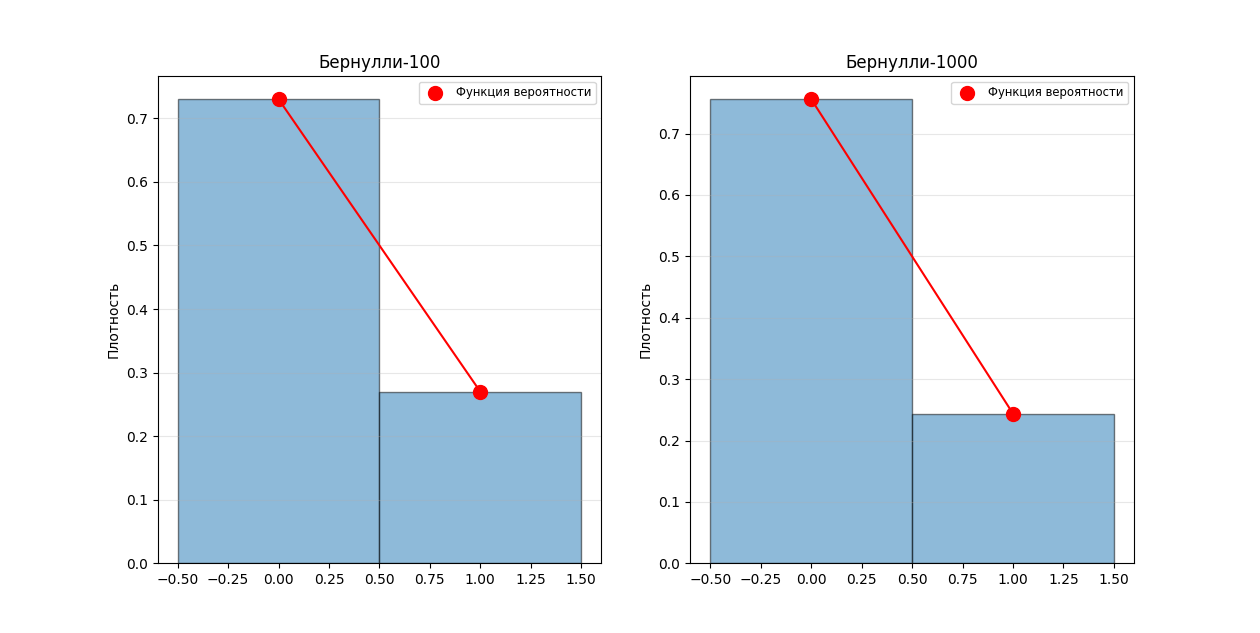
\includegraphics[width=\textwidth]{images/bernoulli.png}
        \label{fig:bernoulli_100}
    \end{figure}

    \subsection{Биномиальное распределение}

    В случае биномиального распределения интервал будет определяться целым числом от 0 до $n$.
    Функция вероятности распределения биномиального распределения имеет вид: \\
    $\displaystyle
    f_X(x) = C_n^x p^x (1 - p)^{n - x}
    $

    Таким образом код будет иметь вид:
    \begin{minted}{python}
        def combinations(n, k) -> float:
            return math.factorial(n) / (math.factorial(k) * math.factorial(n - k))

        def f_x(x: float) -> float:
            return combinations(17, x) * (0.25 ** x) * ((1 - 0.25)**(17 - x))

        fig, axes = plt.subplots(1, 2)

        for col, size in enumerate([100, 1000]):
            ax = axes[col]
            sample = data["binom"][size]["X"]

            k = np.arange(0, 17 + 1)
            counts = [np.sum(sample == i) for i in k]

            heights = [m_i / size for m_i in counts]

            ax.bar(k, heights, width=h, alpha=0.5, edgecolor='black')

            ax.scatter(k, [f_x(i) for i in k], s=100, zorder=5, label='Функция вероятности', color="red")
            ax.plot(k, [f_x(i) for i in k], color="red")

            ax.set_title(f"Биномиальное-{size}")
            ax.set_ylabel("Плотность")
            ax.legend(fontsize='small')
            ax.grid(axis='y', alpha=0.3)
    \end{minted}

    Графики получились такими:
    \begin{figure}[ht!]
        \centering
        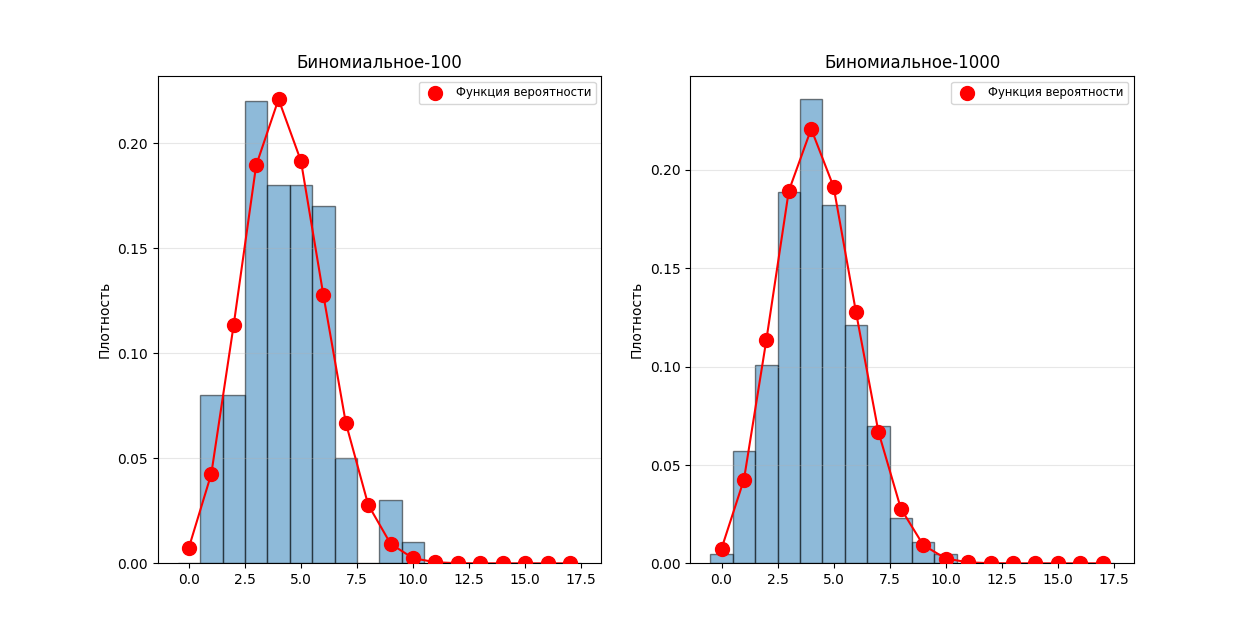
\includegraphics[width=\textwidth]{images/binom.png}
        \label{fig:binom_100}
    \end{figure}

    \subsection{Нормальное распределение}

    Плотность вероятности для нормального распределения имеет вид:
    $\displaystyle
    f_X(x) = \frac{1}{\sigma \sqrt{2 \pi}} e^{-\frac{(x - M)^2}{2 \sigma^2}}
    $

    Код аналогичен равномерному распределению:
    \begin{minted}{python}
        def f_x(x: float) -> float:
            return 1 / (5 * np.sqrt(2 * np.pi)) * np.exp(-(x - 15) ** 2 / (2 * 5 ** 2))

        fig, axes = plt.subplots(1, 2)

        for col, size in enumerate([100, 1000]):
            ax = axes[col]
            sample = data["norm"][size]["X"]

            k = int(1 + 3.322 * np.log10(len(sample)))
            h = (max(sample) - min(sample)) / k

            endpoints = np.linspace(min(sample), max(sample), k + 1)
            heights = []
            for i in range(k):
                left = endpoints[i]
                right = endpoints[i+1]
                count = ((sample >= left) & (sample < right)).sum()
                
                density_height = count / (size * h)
                heights.append(density_height)

            bin_centers = endpoints[:-1] + h / 2
            ax.bar(bin_centers, heights, width=h, alpha=0.5, edgecolor='black')

            k = np.linspace(min(sample), max(sample), 100)
            ax.plot(k, [f_x(i) for i in k], 'r-', lw=2.5, label='Плотность вероятностей')

            ax.set_title(f"Нормальное-{size}")
            ax.set_ylabel("Плотность")
            ax.legend(fontsize='small')
            ax.grid(axis='y', alpha=0.3)
    \end{minted}

    График вышел таким:
    \begin{figure}[ht!]
        \centering
        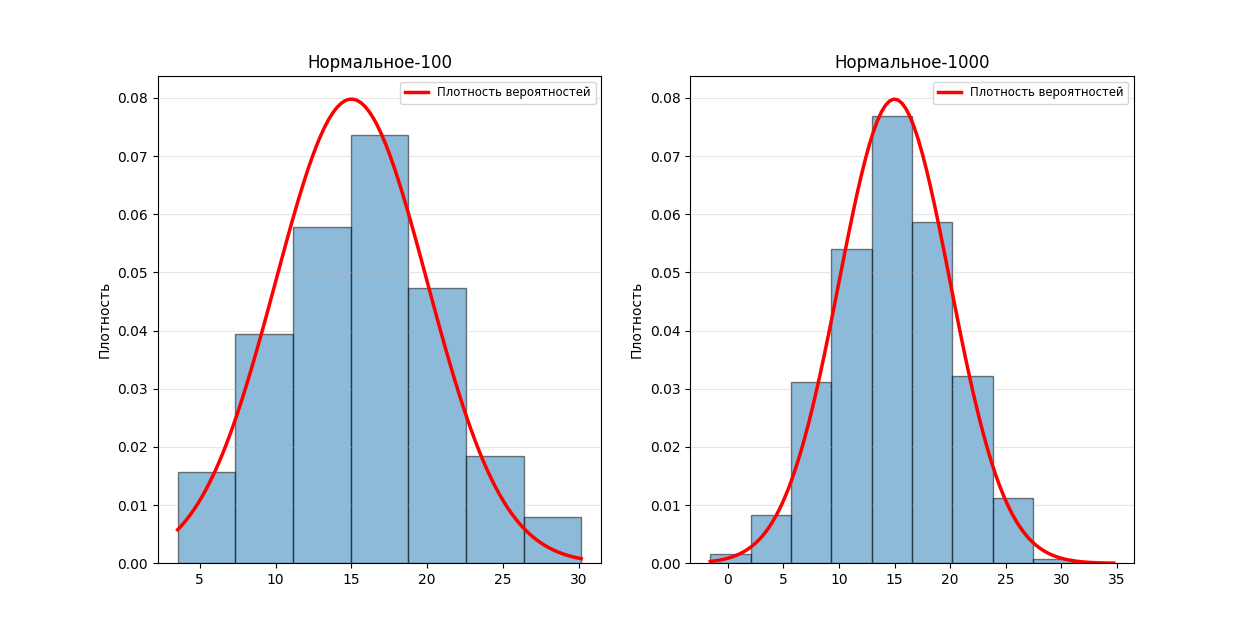
\includegraphics[width=\textwidth]{images/norm.png}
        \label{fig:norm_100}
    \end{figure}

\end{document}